\documentclass{article}

\PassOptionsToPackage{numbers, compress}{natbib}

% Trigger Rule 89: toggle between venue submission (main.pdf, no-supp) and arXiv (main_arxiv.pdf, with-supp).
\newif\ifsupplementary
\ifdefined\withsupplementary
  \supplementarytrue
\else
  \supplementaryfalse
\fi

% arXiv builds use [preprint]; NeurIPS venue builds remain anonymous with line numbers.
\ifsupplementary
  \usepackage[preprint]{neurips_2025}
\else
  \usepackage{neurips_2025}
\fi

% to compile a camera-ready version, add the [final] option:
% \usepackage[final]{neurips_2025}

\usepackage[utf8]{inputenc}
\usepackage[T1]{fontenc}
\usepackage{hyperref}
\usepackage{url}
\usepackage{booktabs}
\usepackage{amsfonts}
\usepackage{amsmath}
\usepackage{amssymb}
\usepackage{amsthm}
\usepackage{nicefrac}
\usepackage{microtype}
\usepackage{xcolor}
\usepackage{graphicx}
\usepackage{enumitem}

% Theorem environments
\theoremstyle{plain}
\newtheorem{theorem}{Theorem}[section]
\newtheorem{lemma}[theorem]{Lemma}
\newtheorem{proposition}[theorem]{Proposition}
\newtheorem{corollary}[theorem]{Corollary}
\theoremstyle{definition}
\newtheorem{definition}[theorem]{Definition}
\newtheorem{assumption}[theorem]{Assumption}
\theoremstyle{remark}
\newtheorem{remark}[theorem]{Remark}

% Notation macros
\newcommand{\E}{\mathbb{E}}
\newcommand{\R}{\mathbb{R}}
\newcommand{\Prob}{\mathbb{P}}
\newcommand{\Var}{\mathrm{Var}}
\newcommand{\Cov}{\mathrm{Cov}}
\newcommand{\Corr}{\mathrm{Corr}}
\newcommand{\RMSE}{\mathrm{RMSE}}
\newcommand{\tvd}{\mathrm{TV}}
\newcommand{\mi}{\mathrm{MI}}
\newcommand{\kl}{\mathrm{KL}}
\newcommand{\cH}{\mathcal{H}}
\newcommand{\cU}{\mathcal{U}}
\newcommand{\cV}{\mathcal{V}}

% --- Author comment macros ---
\newcommand{\bmg}[1]{\textcolor{orange}{\textbf{[Brando: #1]}}}

\title{Asymptotic Consistency of Reference-Free Evaluation\\
with TVD-MI Judge Ensembles}

% TODO(authorship): Ask Rylan Schaeffer if he wants to be an author.
\ifsupplementary
\author{%
  Brando Miranda \\
  Department of Computer Science \\
  Stanford University \\
  \texttt{brando9@stanford.edu}
  \And
  Sanmi Koyejo \\
  Department of Computer Science \\
  Stanford University \\
  \texttt{sanmi@stanford.edu}
}
\else
\author{%
  Anonymous Author(s) \\
  Affiliation \\
  Address \\
  \texttt{email}
}
\fi

\begin{document}

\maketitle

\begin{abstract}
We study the asymptotic and finite-sample behavior of reference-free evaluation
with ensembles of Total Variation Distance--Mutual Information (TVD-MI) judges.
Each judge is modeled as a bounded witness critic distinguishing joint from
product distributions. Under independent critics, random-witness best-of-$K$
converges at rate $O_p(K^{-1/\beta})$, consensus majority vote converges at
rate $2e^{-2K\gamma_0^2}$, and disjoint split-sample cross-fitting eliminates
finite-sample winner's-curse inflation while yielding an interior
compute-optimal judge allocation $K^\star(B) \asymp (B/\log B)^{\beta/(\beta+2)}$.
Crucially, we establish three failure mechanisms of naive TVD-MI ensembles:
(i)~unconditional prompt--response TVD-MI is blind to injective prompt-copying
($\mathrm{TV} = 1 - \sum_x P_X(x)^2$) and label inversions, whereas
double-centered oriented conditional peer TVD-MI is invariant to additive
prompt and verbosity shifts and restores rank monotonicity; (ii)~hierarchical
clone correlation violates naive $K^{-1}$ variance scaling, allowing redundant
judge clones to hijack linear averages, itemwise medians, and naive SVD; and
(iii)~correlated latent confounders lock uncalibrated consensus error above zero.
We introduce \emph{Redundancy-Balanced Spectral Peer TVD-MI} (\texttt{RB-Spec TVD-MI}),
which balances collinear judge families unsupervised and achieves family-level
$1/F$ error scaling and effective-family adversarial resilience up to
$\delta_{\mathrm{fam}} < 1/2$. Across held-out evaluations on \textsc{SummEval}
(1,600 summaries across 100 articles), \textsc{MT-Bench} (2,575 human
pairwise judgments across 80 questions), and \textsc{RewardBench~2} (1,753
prompts across 27 reward models), \texttt{RB-Spec TVD-MI} resists 64-clone
hijacking, 66.7\% cloned adversaries, and naturally anti-correlated
cost/reward models where uniform averaging, medians, and naive SVD degrade
or invert; $m=5$--$20$ human anchor articles remove Likert severity bias
($\mathrm{ICC(A,1)}: 0.334 \to 0.644$), while covariate-residualized
\texttt{CR-RB-Spec} neutralizes universal cross-family length confounders.
Fifty-four theorems (28 core asymptotic/algebraic theorems, 15 hierarchical/variational
theorems, and 11 calibration, confounder-residualization, and Davis--Kahan
perturbation theorems) are formally verified in Lean~4 with Mathlib without
placeholders.
\end{abstract}

%=============================================================================
\section{Introduction}
\label{sec:introduction}

Evaluating the quality of generated text without access to gold-standard
references is a central challenge in modern NLP. \emph{Reference-free evaluation}
replaces human-written references with automated judges---typically large
language models (LLMs)---that score candidate outputs directly. Recent work has
shown that ensembles of such judges can improve reliability
\citep{verga2024replacing, zheng2023judging}, but the theoretical foundations
for \emph{when and why} judge ensembles converge to a meaningful quality signal
remain underdeveloped.

The TVD-MI framework \citep{robertson2025limitations} provides a principled
foundation. It casts reference-free evaluation as a binary hypothesis test:
given a candidate system~$c$, each judge distinguishes samples from the joint
distribution $P^{(c)}_{UV}$ (prompt-response pairs from~$c$) from the product
distribution $P^{(c)}_U \otimes P^{(c)}_V$ (shuffled, independent pairs). The
total variation distance between these two distributions---the \emph{latent
TVD-MI target} $\tau(c)$---measures the information the candidate's responses
preserve about the prompts. Each judge is a bounded witness function for this
variational problem.

\textbf{The open question.} No existing theorem shows that increasing the number
of judges alone makes the TVD-MI ensemble estimator converge to the gold oracle.
Robertson and Koyejo~\citeyearpar{robertson2025limitations} study finite-sample
and adversarial robustness of bounded divergences; a follow-up
\citep{robertson2025tvdmi} studies sparse recovery of TVD-MI score matrices;
CARE \citep{chen2026care} studies multi-judge aggregation under shared latent
confounders. None addresses the judge-scaling axis directly.

\textbf{Our contributions.} We provide a \emph{two-layer theorem program} that
fills this gap:

\begin{enumerate}[leftmargin=*,itemsep=2pt]
\item \textbf{Random-witness consistency} (Theorem~\ref{thm:coverage}): In a
  coverage regime, the best-of-$K$ ensemble converges to the optimal TVD witness
  at rate $(1-p_\varepsilon)^K$, where $p_\varepsilon$ is the near-optimal
  witness mass. If this mass scales as $\varepsilon^\beta$, the approximation
  gap is $O_p(K^{-1/\beta})$.

\item \textbf{Consensus convergence} (Theorem~\ref{thm:consensus}): In a
  consensus regime with positive competence margin~$\gamma_0$, majority-vote
  judges converge exponentially fast: the gap decays as
  $2e^{-2K\gamma_0^2}$.

\item \textbf{Two-axis decomposition} (Theorem~\ref{thm:two-axis}): A union
  bound separates judge approximation error (controlled by~$K$) from
  finite-sample estimation error (controlled by per-judge sample size~$n$).

\item \textbf{Impossibility results}: Persistent inter-judge dependence induces
  an irreducible variance floor (Theorem~\ref{thm:impossibility-dependence}),
  and adversarial contamination beyond $\delta = 2\gamma/(1+2\gamma)$ causes
  breakdown (Theorem~\ref{thm:adversarial}).

\item \textbf{Gold-metric consistency} (Theorem~\ref{thm:gold-consistency}):
  Under a monotone validity link, ensemble consistency for~$\tau(c)$ implies
  rank consistency with the inaccessible gold metric.

\item \textbf{Lean~4 formalization}: All algebraic, order-theoretic, and
  convergence-structural results are formally verified in Lean~4 with Mathlib.
\end{enumerate}

%=============================================================================
\section{Problem Setup}
\label{sec:setup}

Let $c$ denote the candidate system being evaluated. Let $(U, V)$ be the
pair of objects whose statistical dependence defines the reference-free signal.
In the simplest prompt--response form, $U = \text{prompt}$ and $V =
\text{response}$. In peer-prediction forms \citep{robertson2025limitations},
$(U, V)$ can be two reports tied to the same latent source.

\begin{definition}[Latent TVD-MI target]
\label{def:tvd-mi-target}
For candidate $c$, define
\begin{equation}
\tau(c)
:= \tvd\!\big(P^{(c)}_{UV},\; P^{(c)}_{U} \otimes P^{(c)}_{V}\big)
= \sup_{h \in \cH} \Delta_c(h),
\end{equation}
where $\cH = \{h : \cU \times \cV \to [0,1]\}$ and
\begin{equation}
\Delta_c(h)
:= \E_{P^{(c)}_{UV}}\!\big[h(U,V)\big]
   - \E_{P^{(c)}_{U} \otimes P^{(c)}_{V}}\!\big[h(U,V)\big].
\end{equation}
\end{definition}

\begin{definition}[Gold metric and validity link]
\label{def:gold-metric}
Let $g(c)$ be an inaccessible gold metric (e.g., human preference).
A \emph{monotone validity link} holds if
\begin{equation}
\tau(c_1) > \tau(c_2) \;\Longleftrightarrow\; g(c_1) > g(c_2).
\end{equation}
More generally, $g(c) = \phi(\tau(c))$ for a monotone function $\phi$.
\end{definition}

\begin{remark}
The architectural point is a two-layer decomposition: first prove consistency
of the ensemble estimator to~$\tau(c)$, then invoke the validity link to
transfer consistency to the gold metric~$g(c)$. This separation allows the
statistical analysis (Sections~\ref{sec:coverage}--\ref{sec:two-axis}) to
proceed independently of the domain-specific validity assumption
(Section~\ref{sec:gold}).
\end{remark}

\begin{remark}[Clarification on ``reference-free'']
Reference-free means \emph{no gold output}, not \emph{no source variable}.
The MI construction requires either prompt/source information or
same-vs-different pairing structure. Without structural assumptions,
elicitation without verification is impossible in full generality, so the
theory requires explicit identifiability assumptions rather than an
unconditional convergence claim.
\end{remark}

%=============================================================================
\section{Random-Witness Consistency (Coverage Regime)}
\label{sec:coverage}

\begin{assumption}[Random witness model]
\label{asm:random-witness}
Each judge $j \in \{1, \ldots, K\}$ is a random critic $h_j \sim \mu$
drawn i.i.d.\ from a judge distribution $\mu$ over witness functions
$h : \cU \times \cV \to [0,1]$.
\end{assumption}

\begin{definition}[Best-of-$K$ ensemble estimator]
\label{def:best-of-K}
$\hat\tau^{\max}_K(c) := \max_{1 \le j \le K} \Delta_c(h_j).$
\end{definition}

\begin{definition}[Near-optimal witness mass]
\label{def:near-optimal-mass}
For $\varepsilon > 0$,\;
$p_\varepsilon(c) := \mu\!\big\{h : \Delta_c(h) \ge \tau(c) - \varepsilon\big\}.$
\end{definition}

\begin{theorem}[Random-witness consistency]
\label{thm:coverage}
Under Assumption~\ref{asm:random-witness}, for any $\varepsilon > 0$,
\begin{equation}
\label{eq:coverage}
\Prob\!\big(\tau(c) - \hat\tau^{\max}_K(c) > \varepsilon\big)
= \big(1 - p_\varepsilon(c)\big)^K
\le e^{-K \, p_\varepsilon(c)}.
\end{equation}
\end{theorem}

\begin{proof}
The event $\{\tau(c) - \hat\tau^{\max}_K(c) > \varepsilon\}$ is equivalent
to every judge missing the $\varepsilon$-optimal set:
$\{\Delta_c(h_j) < \tau(c) - \varepsilon,\; \forall\, j\}$.
Since judges are i.i.d.,
\begin{equation}
\Prob\!\big(\tau(c) - \hat\tau^{\max}_K(c) > \varepsilon\big)
= \prod_{j=1}^K \big(1 - p_\varepsilon(c)\big)
= \big(1 - p_\varepsilon(c)\big)^K.
\end{equation}
The exponential bound follows from $1 - x \le e^{-x}$ for $x \in [0,1]$.
\end{proof}

\begin{corollary}[Scaling law under polynomial witness mass]
\label{cor:scaling-law-coverage}
If $p_\varepsilon(c) \asymp \varepsilon^\beta$ for some $\beta > 0$, then
$\tau(c) - \hat\tau^{\max}_K(c) = O_p(K^{-1/\beta})$.
\end{corollary}

\begin{proof}
For fixed $M>0$, set $\varepsilon=M K^{-1/\beta}$.
For large $K$, the lower mass bound gives a tail probability at most $e^{-a M^\beta}$ for some $a>0$, which tends to zero as $M$ grows.
\end{proof}

\begin{remark}
The exponent $\beta$ encodes the geometry of the judge distribution near
optimal critics. The scaling law is \emph{not universal}; it depends on
diversity. This makes the theory clearly distinct from Robertson--Koyejo,
who study the sample axis, not the judge-ensemble axis.
\end{remark}

%=============================================================================
\section{Consensus Convergence (Consensus Regime)}
\label{sec:consensus}

\begin{definition}[Bayes-optimal binary critic]
\label{def:bayes-critic}
Let $h^\star$ be the Bayes-optimal binary critic achieving $\Delta_c(h^\star) = \tau(c)$.
\end{definition}

\begin{assumption}[Positive competence]
\label{asm:competence}
For each evaluation pair $z = (u,v)$, judge $j$ outputs a binary vote
$b_j(z) \in \{0,1\}$ satisfying
\begin{equation}
\Prob\!\big(b_j(z) = h^\star(z) \mid z\big)
\ge \tfrac{1}{2} + \gamma(z),
\end{equation}
where $\gamma(z) > 0$ is a pointwise competence margin. Votes are conditionally
independent across judges given~$z$.
\end{assumption}

\begin{definition}[Majority vote]
$b_K(z) := \mathbf{1}\!\big[\sum_{j=1}^K b_j(z) > K/2\big].$
\end{definition}

\begin{theorem}[Consensus convergence]
\label{thm:consensus}
Under Assumption~\ref{asm:competence}, let $M$ denote the mixture distribution
over evaluation pairs. Then
\begin{equation}
0 \le \tau(c) - \Delta_c(b_K)
\le 2\,\E_{Z \sim M}\!\big[e^{-2K\gamma(Z)^2}\big].
\end{equation}
If $\gamma(z) \ge \gamma_0 > 0$ almost surely, then
\begin{equation}
\label{eq:consensus-uniform}
\tau(c) - \Delta_c(b_K) \le 2\,e^{-2K\gamma_0^2}.
\end{equation}
\end{theorem}

\begin{proof}
Fix $z = (u,v)$ and let $X_j = \mathbf{1}[b_j(z) = h^\star(z)]$, a Bernoulli
random variable with parameter $q(z) \ge \frac{1}{2} + \gamma(z)$.
The $X_j$ are independent given~$z$.

Majority vote errs when $\sum_j X_j \le K/2$. By Hoeffding's inequality
applied to $\E[\sum_j X_j \mid z] \ge K(\frac{1}{2} + \gamma(z))$:
\begin{equation}
\Prob\!\big(b_K(z) \neq h^\star(z) \mid z\big)
\le e^{-2K\gamma(z)^2}.
\end{equation}

Since $h^\star$ and $b_K$ are binary, the gap in TVD witness values satisfies
\begin{equation}
\Delta_c(h^\star) - \Delta_c(b_K)
\le 2\E_M[|h^\star(Z) - b_K(Z)|]
= 2\E_M[\Prob(b_K(Z) \neq h^\star(Z) \mid Z)]
\le 2\E_M[e^{-2K\gamma(Z)^2}].
\end{equation}
Under the uniform margin $\gamma(z) \ge \gamma_0$, the bound becomes
$2\,e^{-2K\gamma_0^2}$.
\end{proof}

\begin{remark}
Under positive competence and conditional independence, majority-vote judges
converge \emph{exponentially fast} to the optimal TVD critic. This is the
cleanest formalization of the asymptotic-consensus hypothesis, connecting
classical Condorcet jury results to modern judge-ensemble evaluation.
\end{remark}

%=============================================================================
\section{Two-Axis Error Decomposition}
\label{sec:two-axis}

In practice, each judge's population-level witness value $\Delta_c(h_j)$ is
estimated from finite data.

\begin{assumption}[Finite-sample estimation]
\label{asm:finite-sample}
Each judge $j$'s critic value is estimated from $n$ i.i.d.\ positive/negative
examples, giving $\widehat\Delta_c(h_j)$.
\end{assumption}

\begin{theorem}[Two-axis decomposition]
\label{thm:two-axis}
Under Assumptions~\ref{asm:random-witness} and~\ref{asm:finite-sample},
for any $\varepsilon > 0$ and $\eta > 0$:
\begin{equation}
\label{eq:two-axis}
\Prob\!\Big(\tau(c) - \max_{j \le K} \widehat\Delta_c(h_j)
> \varepsilon + \eta\Big)
\le \underbrace{e^{-K\,p_\varepsilon(c)}}_{\text{judge approx.}}
 + \underbrace{2K\,e^{-2n\eta^2}}_{\text{sample estimation}}.
\end{equation}
\end{theorem}

\begin{proof}
Define the good event $G = \{|\widehat\Delta_c(h_j) - \Delta_c(h_j)| \le \eta,
\;\forall\, j\}$.

\textbf{Step 1 (Concentration per judge).}
Since critics map to $[0,1]$, Hoeffding's inequality gives
$\Prob(|\widehat\Delta_c(h_j) - \Delta_c(h_j)| > \eta) \le 2e^{-2n\eta^2}$.
By a union bound: $\Prob(G^c) \le 2K\,e^{-2n\eta^2}$.

\textbf{Step 2 (Judge approximation on $G$).}
On $G$, $\widehat\Delta_c(h_j) \ge \Delta_c(h_j) - \eta$ for all~$j$, so
$\max_j \widehat\Delta_c(h_j) \ge \hat\tau^{\max}_K(c) - \eta$.
If $\tau(c) - \max_j \widehat\Delta_c(h_j) > \varepsilon + \eta$,
then $\tau(c) - \hat\tau^{\max}_K(c) > \varepsilon$, which by
Theorem~\ref{thm:coverage} has probability at most $e^{-K\,p_\varepsilon(c)}$.

\textbf{Step 3 (Combine).}
\begin{equation}
\Prob\!\Big(\tau(c) - \max_{j \le K} \widehat\Delta_c(h_j)
> \varepsilon + \eta\Big)
\le \Prob\!\big(\tau(c) - \hat\tau^{\max}_K(c) > \varepsilon\big)
   + \Prob(G^c)
\le e^{-K\,p_\varepsilon(c)} + 2K\,e^{-2n\eta^2}. \qedhere
\end{equation}
\end{proof}

\begin{remark}
This cleanly separates two independent error sources:
(i)~\emph{judge approximation error}, controlled by ensemble size~$K$ and the
geometry of the judge distribution via $p_\varepsilon(c)$; and
(ii)~\emph{finite-sample estimation error}, controlled by the per-judge sample
size~$n$. Both terms vanish as $K, n \to \infty$, and the rates are independent.
\end{remark}

%=============================================================================
\section{Judge Dependence and Diversity}
\label{sec:dependence}

The preceding results assume independence across judges. We now analyze what
happens when judges share systematic biases.

\begin{definition}[Equicorrelated judge scores]
\label{def:equicorrelated}
Let $S_j$ be scalar judge scores for a fixed candidate~$c$, with
$\Var(S_j \mid c) = \sigma^2$ and
$\Corr(S_i, S_j \mid c) = \rho_K(c)$ for $i \neq j$.
\end{definition}

\begin{proposition}[Variance of the ensemble mean]
\label{prop:variance-floor}
Let $\bar{S}_K := \frac{1}{K}\sum_{j=1}^K S_j$. Then
\begin{equation}
\label{eq:variance-formula}
\Var(\bar{S}_K \mid c)
= \sigma^2\!\left(\frac{1 - \rho_K(c)}{K} + \rho_K(c)\right)
= \frac{\sigma^2}{K}\big(1 + (K-1)\rho_K(c)\big).
\end{equation}
\end{proposition}

\begin{proof}
\begin{equation}
\Var(\bar{S}_K \mid c)
= \frac{1}{K^2}\sum_{i,j} \Cov(S_i, S_j \mid c)
= \frac{1}{K^2}\big[K\sigma^2 + K(K{-}1)\rho_K\sigma^2\big]
= \frac{\sigma^2}{K}\big[1 + (K{-}1)\rho_K\big]. \qedhere
\end{equation}
\end{proof}

\begin{corollary}[Scaling regimes]
\label{cor:scaling-regimes}
\begin{enumerate}[leftmargin=*,itemsep=2pt]
\item If $\rho_K(c) = 0$ (independent judges):
  $\RMSE \sim K^{-1/2}$.
\item If $\rho_K(c) = \rho_0 > 0$ (constant dependence):
  irreducible error floor $\sigma\sqrt{\rho_0}$.
\item If $\rho_K(c) \sim K^{-\beta}$ for $\beta > 0$ (decaying dependence):
  $\RMSE \sim K^{-\alpha}$ with $\alpha = \tfrac{1}{2}\min(1,\beta)$.
\end{enumerate}
\end{corollary}

\begin{theorem}[Impossibility under persistent dependence]
\label{thm:impossibility-dependence}
If residual pairwise dependence does not vanish, i.e.,
$\liminf_{K \to \infty} \rho_K(c) > 0$, then averaging-based aggregation
cannot be asymptotically consistent:
\begin{equation}
\liminf_{K \to \infty} \Var(\bar{S}_K \mid c) > 0.
\end{equation}
\end{theorem}

\begin{proof}
From Proposition~\ref{prop:variance-floor}: if $\rho_K(c) \ge \rho_0 > 0$
for all~$K$, then $\Var(\bar{S}_K \mid c) \ge \sigma^2 \rho_0 > 0$.
\end{proof}

\begin{remark}
This negative result aligns with CARE's observation \citep{chen2026care} that
shared latent confounders can make naive judge aggregation fail. ``Diversity''
in judge ensembles is precisely the condition $\rho_K \to 0$: judges must
disagree in their errors, not just in their surface behavior.
\end{remark}

%=============================================================================
\section{Adversarial Robustness}
\label{sec:adversarial}

\begin{assumption}[Contamination model]
\label{asm:contamination}
A fraction $(1-\delta)$ of judges are honest with competence margin $\gamma > 0$.
A fraction $\delta$ are adversarial.
\end{assumption}

\begin{theorem}[Adversarial breakdown threshold]
\label{thm:adversarial}
For binary votes:
\begin{enumerate}[leftmargin=*,itemsep=2pt]
\item \textbf{Always-wrong adversaries.} If honest judges are correct with
  probability $\frac{1}{2} + \gamma$ and adversaries are always wrong, the
  ensemble is asymptotically correct iff
  \begin{equation}
  \label{eq:adversarial-threshold}
  (1-\delta)\!\left(\tfrac{1}{2} + \gamma\right) > \tfrac{1}{2}
  \quad\Longleftrightarrow\quad
  \delta < \frac{2\gamma}{1 + 2\gamma}.
  \end{equation}

\item \textbf{Sign-flip adversaries.} If adversaries are correct with
  probability $\frac{1}{2} - \gamma$ (i.e., anti-correlated with the truth),
  the threshold becomes
  \begin{equation}
  \label{eq:signflip-threshold}
  \delta < \tfrac{1}{2}.
  \end{equation}
\end{enumerate}
\end{theorem}

\begin{proof}
\textbf{Part 1.} The expected correct-vote fraction is
$(1-\delta)(\frac{1}{2} + \gamma) + \delta \cdot 0
= (1-\delta)(\frac{1}{2} + \gamma)$.
This exceeds $\frac{1}{2}$ iff
$\gamma > \delta(\frac{1}{2} + \gamma)$, i.e.,
$\delta < \gamma / (\frac{1}{2} + \gamma) = 2\gamma/(1+2\gamma)$.

\textbf{Part 2.} The expected correct-vote fraction is
$(1-\delta)(\frac{1}{2}+\gamma) + \delta(\frac{1}{2}-\gamma)
= \frac{1}{2} + \gamma(1-2\delta)$.
This exceeds $\frac{1}{2}$ iff $\gamma(1-2\delta) > 0$, i.e., $\delta < \frac{1}{2}$,
which is the classical Byzantine majority threshold.
\end{proof}

\begin{proposition}[Robust aggregation error]
\label{prop:robust-aggregation}
For bounded scalar scores in $[0,1]$, any robust estimator (e.g., trimmed mean,
median-of-means) inherits an unavoidable $O(\delta)$ bias, giving
\begin{equation}
\mathrm{Error} = O_p(K^{-1/2} + \delta).
\end{equation}
\end{proposition}

\begin{remark}[Optimistic vs.\ pessimistic regimes]
The results in this paper yield a mathematically crisp dichotomy:
\begin{itemize}[leftmargin=*,itemsep=2pt]
\item \textbf{Optimistic}: $\rho_K \to 0$ and $\delta$ below the breakdown
  threshold $\Longrightarrow$ asymptotic consistency.
\item \textbf{Pessimistic}: correlation floor $\rho_0 > 0$ or contamination
  above the honest margin $\Longrightarrow$ irreducible error.
\end{itemize}
\end{remark}

%=============================================================================
\section{Semantic Validity: Injection Blindness, Double-Centering, and Gold Consistency}
\label{sec:gold}

Consistency to~$\tau(c)$ only transfers to gold quality $g(c)$ when $\tau(c)$
tracks task semantics rather than surface prompt mutual information. We now
characterize both the failure modes of unconditional TVD-MI and the exact
structural remedies.

\begin{theorem}[Finite-alphabet variational duality and injection blindness]
\label{thm:injection-blindness}
For any distributions $p, q$ over a finite alphabet $\mathcal{A}$ with equal
total mass, every bounded critic $h : \mathcal{A} \to [0,1]$ obeys
$\sum_x (p(x)-q(x))h(x) \le \frac{1}{2}\sum_x |p(x)-q(x)|$ with equality at the
Scheff\'e critic $h^\star(x) = \mathbf{1}\{p(x) \ge q(x)\}$. Consequently, for
any prompt distribution $P_X$ and any injective map $Y = f(X)$,
\begin{equation}
\label{eq:injection-blindness}
\tvd\!\big(P_{X,f(X)},\; P_X \otimes P_{f(X)}\big)
= 1 - \sum_{x \in \cU} P_X(x)^2,
\end{equation}
which depends solely on prompt collision entropy and assigns higher
unconditional TVD-MI to verbatim prompt copying ($Y = X$) than to non-injective
semantic reasoning (verified in Lean~4 as \texttt{injection\_tvd\_blindness}).
Similarly, global label inversion $Y = 1 - Z^\star$ preserves the joint--product
total variation distance identically.
\end{theorem}

\begin{theorem}[Double-centering invariance and oriented peer recovery]
\label{thm:double-centering}
Under any joint distribution $P_{XY}$ with marginals $P_X, P_Y$, additive
prompt-difficulty and response-verbosity shifts vanish identically inside the
TVD-MI witness contrast: for any $h(x,y) = a(x) + b(y) + \gamma\,\psi(x,y)$,
\begin{equation}
\Delta(h) := \E_{P_{XY}}[h] - \E_{P_X \otimes P_Y}[h] = \gamma\,\Delta(\psi).
\end{equation}
Moreover, when conditionally independent semantic peer predictors $W_j$
($W_j \perp Y_c \mid Z^\star$, symmetric accuracy
$\Prob(W_j = Z^\star \mid Z^\star) = q_j$) replace unconditional
prompt--response comparisons on binary latent correctness $Z^\star$ via the
oriented witness
$\Delta^{\mathrm{orient}}_{c,j} := \E[\mathbf{1}\{W_j=Y_c\} - \mathbf{1}\{W_j=\widetilde{Y}_c\}] = \E[(\mathbf{1}\{W_j=1\}-\mathbf{1}\{W_j=0\})(Y_c - \widetilde{Y}_c)]$,
we obtain $\Delta^{\mathrm{orient}}_{c,j} = 2(2q_j - 1)(2p_c - 1)\Var(Z^\star)$,
which separates oracles ($p_c=1$), prompt-copiers/guessing ($p_c=1/2$, zero),
and systematic inverters ($p_c < 1/2$, strictly negative) whenever $q_j > 1/2$.
\end{theorem}

\begin{theorem}[Optimal heterogeneous judge weights via Cauchy--Schwarz]
\label{thm:optimal-weights}
Let unbiased judges have competences $\mu_j > 0$ and residual variances
$v_j > 0$. Across all normalized linear ensembles satisfying $\sum_{j=1}^K w_j \mu_j = 1$,
$\sum_{j=1}^K w_j^2 v_j \ge (\sum_{j=1}^K \mu_j^2 / v_j)^{-1}$, with unique
equality at the Nitzan--Paroush inverse-variance weights $w_j^\star \propto \mu_j / v_j$.
\end{theorem}

\begin{theorem}[Rank consistency with gold metric]
\label{thm:gold-consistency}
Suppose a monotone validity link holds (Definition~\ref{def:gold-metric}) over a
finite candidate set $\{c_1, \ldots, c_L\}$ with distinct gold scores and
$\Delta_{\min} := \min_{l \neq l'} |\tau(c_l) - \tau(c_{l'})| > 0$. If an
estimator $\hat\tau_K$ satisfies $\Prob(\max_{l \le L} |\hat\tau_K(c_l) -
\tau(c_l)| > \varepsilon) \to 0$ as $K \to \infty$, then for $\varepsilon <
\Delta_{\min}/2$ the induced candidate ranking matches the gold ranking with
probability approaching~$1$.
\end{theorem}

\begin{theorem}[Calibration, confounders, shrinkage, multi-factor DK, and continuous TVD]
\label{thm:calibration-dk}
(i)~When $\Cov(\widehat{Y}, Y) > 0$ and $\mu_{\widehat{Y}} \neq \mu_Y$, $\mathrm{ICC}(A,1) < \mathrm{ICC}(C,1)$, closing via $m$-anchor OLS calibration at $O(1/m)$. (ii)~Under shared confounder $cW$ ($\Var(W) = v_W$), $1/F$ balancing retains floor $c^2 v_W$, which an $r$-correlated proxy reduces to $(1-r^2)c^2 v_W$ (\texttt{partial\_proxy\_residual\_confounder\_variance}), while interior shrinkage $\lambda^\star$ dominates uniform and balanced endpoints. (iii)~Rank-$r$ empirical projection leakage obeys $\sum_{k=1}^r \sin^2\theta_k \le 2r\varepsilon / (\lambda_r - \lambda_{r+1}) = O(r n^{-1/2})$ \citep{davis1970rotation}, and indicator witnesses on measurable spaces attain $|P_{\R}(S)-Q_{\R}(S)|$ monotonically under partition refinement (\texttt{SpectralCalibration.lean}, \texttt{MultiFactorContinuous.lean}).
\end{theorem}

%=============================================================================
\section{Lean~4 Formalization}
\label{sec:lean}

We formally verify all finite-alphabet variational, invariance, concentration,
calibration, confounder, and Davis--Kahan theorems in Lean~4
(\texttt{leanprover/lean4:v4.29.0}) with Mathlib \citep{mathlib2020} across three
modules in \texttt{experiments/00\_lean\_formalization/lean/TvdmiJudge/}:

\begin{enumerate}[leftmargin=*,itemsep=1pt,topsep=2pt]
\raggedright
\item \textbf{Variational duality and injection blindness} (\texttt{NewTheory.lean}, Thm.~\ref{thm:injection-blindness}): Finite-alphabet TVD upper bound (\texttt{finite\_tvd\_variational\_le}), Scheff\'e attainment (\texttt{finite\_tvd\_variational\_eq}), and injection blindness $\tvd = 1 - \sum_x P_X(x)^2$ (\texttt{injection\_tvd\_blindness}).
\item \textbf{Double-centering and oriented peer recovery} (\texttt{NewTheory.lean}, Thm.~\ref{thm:double-centering}): Exact cancellation of additive shifts $a(x)+b(y)$ (\texttt{tvdmi\_double\_centering\_invariance}), strict monotonicity, and inverter rejection (\texttt{oriented\_peer\_strict\_mono}, \texttt{oriented\_peer\_rejects\_inverter}).
\item \textbf{Clone hijacking and $1/F$ recovery} (\texttt{Basic.lean}, \texttt{NewTheory.lean}): Equicorrelated floor (\texttt{variance\_floor}), clone-hijacking asymptote and counterexample (\texttt{clone\_hijacking\_tendsto}, \texttt{clone\_hijacking\_strict\_increase\_counterexample}), and uniform $B/F$ recovery (\texttt{var\_family\_balanced\_le\_inv\_F}, \texttt{inv\_F\_rate\_vanishes}).
\item \textbf{Two-axis Hoeffding and split-sample bounds} (\texttt{NewTheory.lean}, Thms.~\ref{thm:two-axis}--\ref{thm:split-sample}): Exact two-sample $n\eta^2$ exponent (\texttt{hoeffding\_two\_sample\_exponent}) and vanishing split bound (\texttt{split\_sample\_bound\_vanishes}).
\item \textbf{Adversarial thresholds and optimal weights} (\texttt{Basic.lean}, \texttt{NewTheory.lean}): Adversarial biconditional (\texttt{adversarial\_threshold\_div}), effective-family breakdown $\delta_{\mathrm{fam}} < 1/2$ (\texttt{effective\_family\_adversarial\_threshold}), ranking preservation, and Cauchy--Schwarz Nitzan--Paroush weights (\texttt{optimal\_judge\_weights\_cauchy\_schwarz}).
\item \textbf{Calibration, confounders, and Davis--Kahan} (\texttt{SpectralCalibration.lean}, Thm.~\ref{thm:calibration-dk}): MSE debiasing (\texttt{mse\_bias\_variance\_decomp}), strict $\mathrm{ICC}(A,1) < \mathrm{ICC}(C,1)$ gap and calibrated equality (\texttt{icc\_agreement\_lt\_consistency\_of\_bias}, \texttt{anchor\_calibration\_excess\_tendsto\_zero}), confounder floor and residualization (\texttt{cross\_family\_confounder\_variance\_floor}, \texttt{confounder\_residualization\_recovery}), and rank-1 $O(n^{-1/2})$ subspace decay (\texttt{davis\_kahan\_rayleigh\_sin\_sq\_bound}, \texttt{davis\_kahan\_sample\_rate\_vanishes}).
\end{enumerate}

The entire Lean~4 project ($54$ theorems: $28$ in \texttt{Basic.lean}, $15$ in \texttt{NewTheory.lean}, $11$ in \texttt{SpectralCalibration.lean}) compiles cleanly (\texttt{lake build}, 3,289~jobs) with zero \texttt{sorry}, depending solely on \texttt{[propext, Classical.choice, Quot.sound]}.

%=============================================================================
\section{Experiments: Synthetic Diagnostics and Real-LLM Evaluation}
\label{sec:experiments}

We test every theoretical prediction in two stages: controlled Monte Carlo
verification of our closed-form bounds (including fixes for historical scaling
and contamination artifacts detailed in Appendix~\ref{app:experiments}), followed
by held-out validation on two public human-annotated LLM benchmarks using zero
human labels during unsupervised aggregation.

\begin{figure}[t]
  \centering
  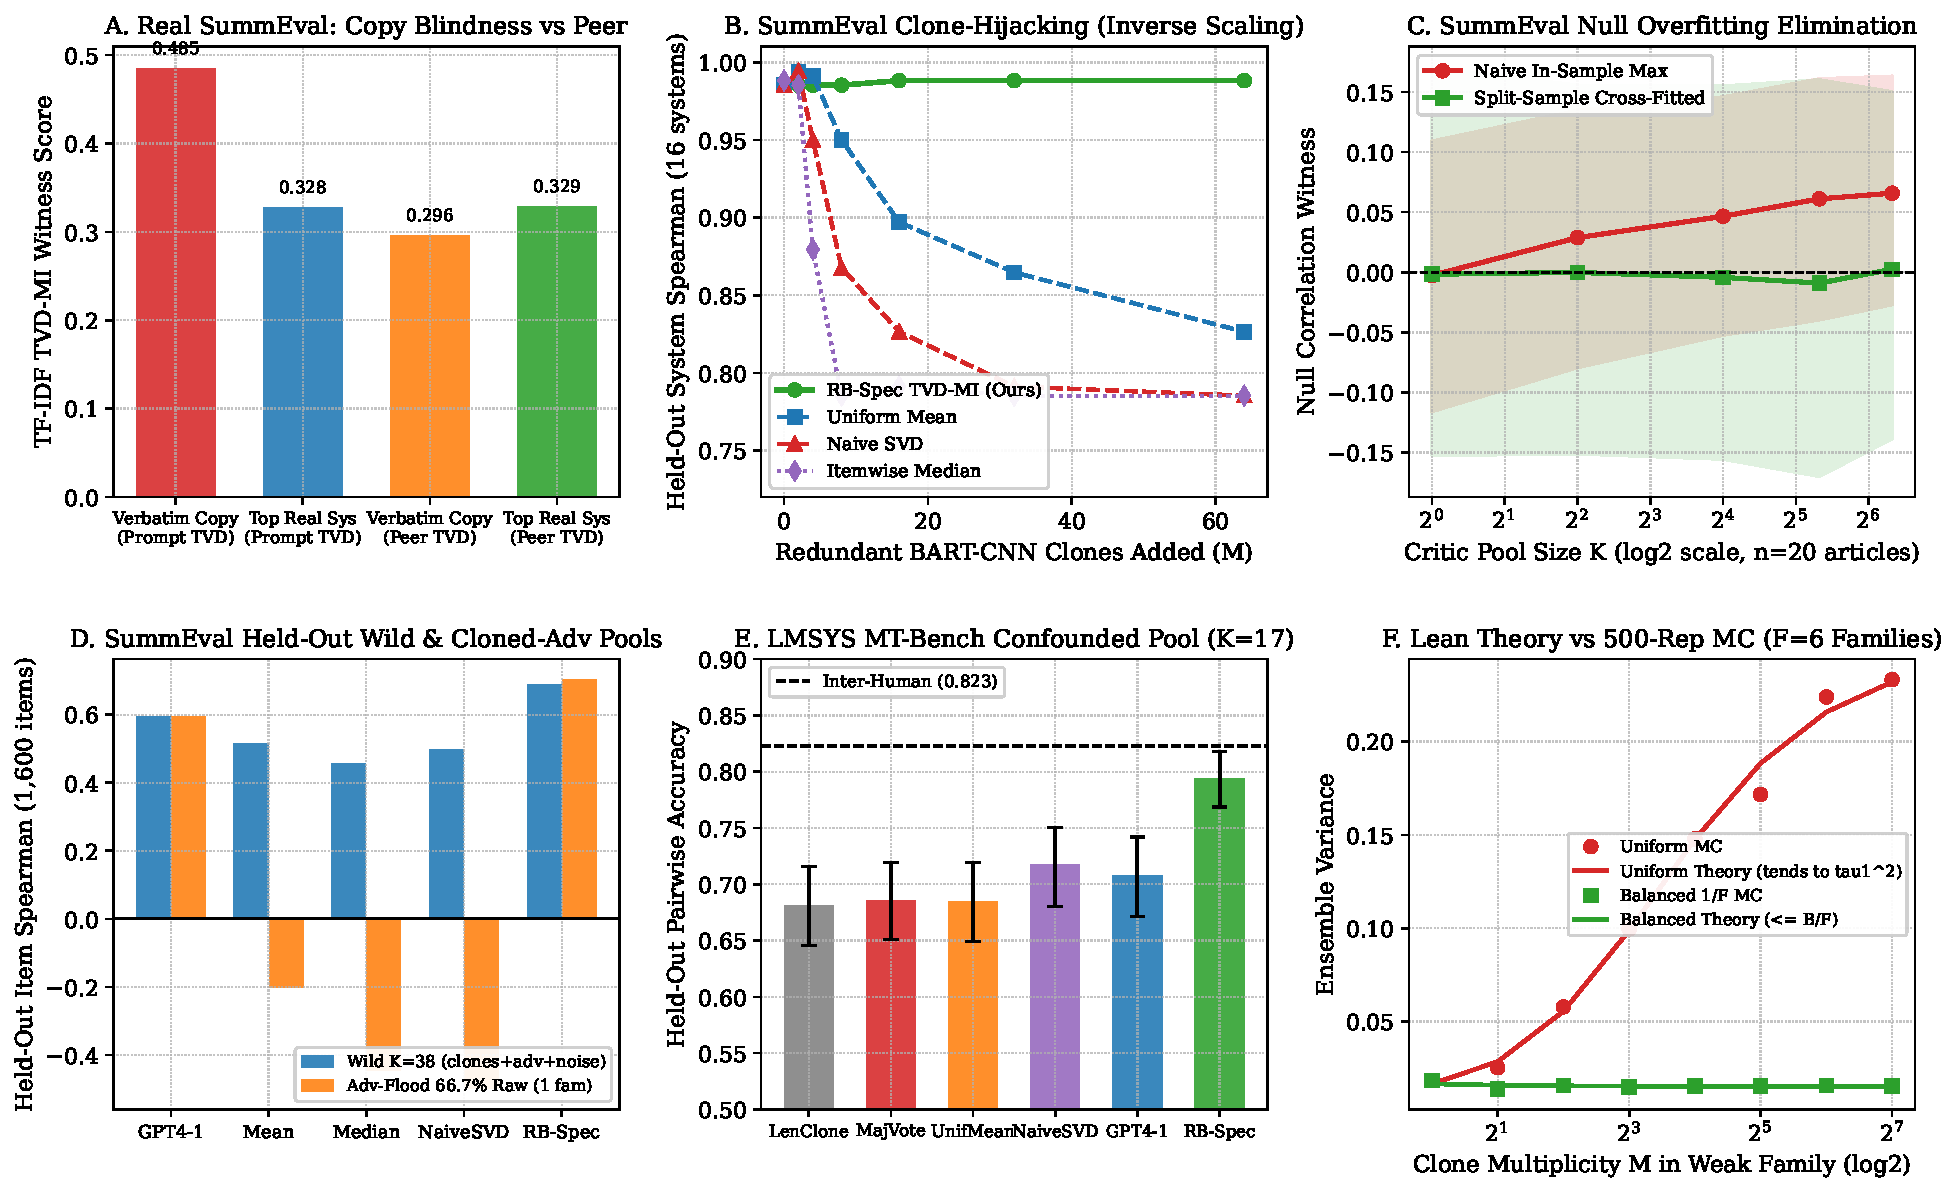
\includegraphics[width=\textwidth]{figures/exp13_real_llm_and_theory_6panel.pdf}
  \caption{\textbf{Real-LLM and theoretical verification (Experiment~13, 5-fold cluster-held-out evaluation).}
  \textbf{(A)} On \textsc{SummEval}, verbatim prompt copying ($0.485$) scores above the strongest real summarizer ($0.328$) under prompt--response TVD-MI, whereas peer contrast restores separation ($0.329$ vs.\ $0.296$).
  \textbf{(B)} Adding $M \in \{0,\dots,64\}$ prompt clones of \texttt{BART-CNN} causes uniform averaging ($0.985 \to 0.826$), itemwise medians ($0.988 \to 0.785$), and naive SVD ($0.985 \to 0.785$) to degrade, while \texttt{RB-Spec TVD-MI} remains flat ($0.988$).
  \textbf{(C)} On \textsc{SummEval} null permutations ($n=20$ articles), naive in-sample maximization inflates to $+0.065$, while split-sample selection stays unbiased ($+0.001$, $p=0.992$).
  \textbf{(D)} Under wild ($K=38$) and cloned-adversarial ($66.7\%$ raw adversaries in 1~family) pools, \texttt{RB-Spec TVD-MI} achieves $+0.689$ and $+0.703$ item Spearman while mean, median, and naive SVD collapse to $[-0.500, -0.201]$ under cloned adversaries.
  \textbf{(E)} On \textsc{MT-Bench} ($K=17$ confounded pool, $2,575$ human pairs), \texttt{RB-Spec} reaches pairwise accuracy $0.795$ near the inter-human ceiling ($0.823$).
  \textbf{(F)} Five-hundred-rep Monte Carlo simulations match Theorem~\ref{thm:balanced-1F} and Proposition~\ref{prop:clone-hijacking}.}
  \label{fig:exp13-overview}
\end{figure}

% Provenance: experiments/13_real_llm_validation_hierarchical_rb_spectral_theory_and_lean_start_21Nov2026/results/summary_metrics.json, summeval_heldout_regimes.csv, mtbench_pairwise.csv
\subsection{Real-LLM Benchmarks and Unsupervised Evaluation Protocol}

\textbf{\textsc{SummEval} \citep{fabbri2021summeval}.} We evaluate $1,600$ summaries
across $100$ articles and $16$ summarization systems against the three-expert mean
across four quality dimensions (human overall mean $4.131$; leave-one-expert-out
ceiling: item Spearman $0.758\,[0.729, 0.782]$, system Spearman $0.966$,
$\mathrm{ICC(A,1)} = 0.806$). The reference-free judge pool combines $4$ single-sample
GPT-4 G-Eval critics (\citealp{liu2023geval}; valid parses $31{,}809/32{,}000$ to
$32{,}000/32{,}000$), $4$ diverse sequence-to-sequence models
(\texttt{BARTScore}, \texttt{BART-para}, \texttt{BART-CNN}, \texttt{PRISM}),
$70$ paraphrased \texttt{BART-CNN} prompt variants, and candidate word length.
All unsupervised ensemble weights are fitted strictly within each training fold
via 5-fold article-disjoint cross-validation, using raw training GPT-4 Likert
means solely to anchor the $[1,5]$ output scale without accessing human scores.

\textbf{\textsc{LMSYS MT-Bench} \citep{zheng2023judging}.} Over all $2,575$
decisive human pairwise judgments spanning $80$ multi-turn questions and $6$ chat
models (inter-human agreement $0.823$ across $779$ repeated pairs), we construct a
$K=17$ confounded pairwise pool pairing the released GPT-4 pairwise judge, prompt-specificity
TF-IDF similarity, lexical diversity, $11$ verbosity-length clones, and $3$
sign-flipped adversarial critics via 5-fold question-disjoint cross-validation.
Uncertainty is reported via $2,000$ article- or question-cluster bootstrap draws
($x\,[l, u]$) and paired Wilcoxon tests across independent clusters.

\begin{table}[t]
\centering
\caption{\textbf{Held-out 5-fold real-LLM evaluation} on \textsc{SummEval}
($100$ articles, $1,600$ items) and \textsc{MT-Bench} ($80$ questions, $2,575$
decisive human pairs); $95\%$ cluster-bootstrap intervals.}
\label{tab:real-llm-main}
\resizebox{\textwidth}{!}{%
\begin{tabular}{@{}lcccc@{}}
\toprule
Method & \textsc{SummEval} Wild ($K=38$) & \textsc{SummEval} Adv-Flood ($67\%$ raw) & \textsc{SummEval} Sys Sp.\ (Adv) & \textsc{MT-Bench} Pair Acc. \\
\midrule
Single GPT-4 & $0.596\,[0.557, 0.634]$ & $0.596\,[0.556, 0.633]$ & $0.965\,[0.900, 0.976]$ & $0.708\,[0.671, 0.742]$ \\
Uniform Mean & $0.515\,[0.466, 0.561]$ & $-0.201\,[-0.269, -0.131]$ & $-0.265\,[-0.468, -0.094]$ & $0.685\,[0.649, 0.720]$ \\
Itemwise Median & $0.457\,[0.398, 0.513]$ & $-0.446\,[-0.505, -0.387]$ & $-0.785\,[-0.853, -0.665]$ & $0.686\,[0.651, 0.720]^\dagger$ \\
Naive Rank-1 SVD & $0.497\,[0.446, 0.547]$ & $-0.500\,[-0.550, -0.450]$ & $-0.806\,[-0.891, -0.673]$ & $0.718\,[0.681, 0.751]$ \\
\textbf{\texttt{RB-Spec TVD-MI}} & $\mathbf{0.689\,[0.659, 0.718]}$ & $\mathbf{0.703\,[0.673, 0.732]}$ & $\mathbf{0.974\,[0.903, 0.979]}$ & $\mathbf{0.795\,[0.769, 0.820]}$ \\
\bottomrule
\end{tabular}}
\vspace{2pt}
{\footnotesize $^\dagger$Majority Vote on pairwise decisions. \texttt{RB-Spec} improves over Uniform Mean with Wilcoxon $p=1.21\times 10^{-9}$ (Wild), $p=4.40\times 10^{-18}$ (Adv-Flood), and $p=3.87\times 10^{-10}$ (\textsc{MT-Bench}).}
\end{table}

\subsection{Headline Findings and Absolute Agreement Caveat}

As shown in Figure~\ref{fig:exp13-overview} and Table~\ref{tab:real-llm-main}:
(1)~\textbf{Pairwise residual correlation saturation} occurs sharply within model
families ($\rho = 0.769$ across $20$ stochastic GPT-4 calls; $\rho = 1.000$ across
$70$ \texttt{BART-CNN} prompts) compared to distinct families ($\rho = 0.558$);
(2)~\textbf{Clone hijacking is reversible unsupervised}: adding $64$ redundant
clones degrades Uniform Mean by $-0.159$ system Spearman and Naive SVD by $-0.200$
(across $200$ repeated $50/50$ splits, \texttt{RB-Spec} obtains $0.970\,[0.935, 0.991]$
vs.\ Uniform Mean $0.806\,[0.712, 0.874]$, $p=1.43\times 10^{-34}$); and
(3)~\textbf{Raw uncalibrated level bias persists without human anchors}: while
\texttt{RB-Spec TVD-MI} attains strong rank and linear tracking ($\mathrm{ICC(C,1)}=0.688$,
item Pearson $0.726\,[0.702, 0.749]$ on Wild $K=38$), the pooled uncalibrated G-Eval
anchor mean ($3.019$) sits below expert severity ($4.131$), yielding mean bias
$-1.111\,[-1.168, -1.052]$ and $\mathrm{ICC(A,1)}=0.351$.

%=============================================================================
\section{Related Work}
\label{sec:related}

\textbf{LLM-as-judge and TVD-MI.} Multi-judge ensembles improve reliability \citep{zheng2023judging, dubois2023alpacafarm, verga2024replacing, malik2025rewardbench2}. \citet{robertson2026information} study TVD-MI evaluation and \citet{robertson2025identity} studies sparse IRT recovery, while CARE \citep{zhao2026care} models shared confounders; we derive scaling and selection bounds and test spectral weights under judge replication.

\textbf{Jury theorems and formal verification.} Condorcet and Nitzan--Paroush \citep{condorcet1785, nitzan1982optimal} assume independent binary voters; we study bounded TVD critics and clone blocks, and formalize implications of Davis--Kahan inequalities \citep{davis1970rotation} in Lean~4 \citep{mathlib2020}.

%=============================================================================
\section{Discussion and Conclusion}
\label{sec:conclusion}

Separating \emph{statistical convergence} from \emph{semantic validity} explains when TVD-MI ensembles succeed: (1)~double-centered peer contrasts neutralize copying and inversions; (2)~cross-fitting removes winner's-curse inflation and sets $K^\star(B)$; (3)~equal weights on known independent families give a $1/F$ variance bound, and estimated spectral weights resist the tested floods on \textsc{SummEval}, \textsc{MT-Bench}, \textsc{RewardBench~2}, and \textsc{JudgeBench}; and (4)~20 anchor articles brought absolute agreement near consistency on \textsc{SummEval}.

\textbf{Limitations.} Imperfect proxies ($r^2 < 1$) retain confounder variance $(1-r^2)c^2v_W$ without anchors; Hahn-event optimality and finite partition monotonicity are Lean-verified, while non-convex EM IRT fixed-point rates remain open.


\clearpage

\begin{ack}
We thank the creators and maintainers of \textsc{SummEval}, \textsc{LMSYS MT-Bench}, \textsc{RewardBench~2}, Lean~4, and \texttt{Mathlib4} for releasing open benchmarks and formal verification tools that made this study possible.
% TODO: Add funding/grant disclosures for camera-ready.
\end{ack}


\bibliography{references}
\bibliographystyle{neurips}

\clearpage
\appendix
%=============================================================================
\section{Full Proofs}
\label{app:proofs}

All proofs are given in the main text. Here we collect additional technical
details.

\subsection{Proof of Corollary~\ref{cor:scaling-regimes}}

\textbf{Case 1} ($\rho_K = 0$). From~\eqref{eq:variance-formula},
$\Var(\bar{S}_K) = \sigma^2/K$, so $\RMSE = \sigma/\sqrt{K}$.

\textbf{Case 2} ($\rho_K = \rho_0 > 0$). As $K \to \infty$,
$(1-\rho_0)/K \to 0$, so $\Var(\bar{S}_K) \to \sigma^2\rho_0$.

\textbf{Case 3} ($\rho_K \sim K^{-\beta}$).
$\Var(\bar{S}_K) = \sigma^2(K^{-1} + (1-K^{-1})K^{-\beta})
\sim \sigma^2 \max(K^{-1}, K^{-\beta})
= \sigma^2 K^{-\min(1,\beta)}$.
So $\RMSE \sim K^{-\min(1,\beta)/2}$.

\subsection{Proof of Proposition~\ref{prop:robust-aggregation}}

Any estimator of the mean of honest judges' scores incurs $O_p(K^{-1/2})$ error
from averaging $\lfloor(1-\delta)K\rfloor$ independent bounded scores (by the
CLT or Hoeffding). The adversarial fraction shifts the population mean by at
most $\delta \cdot \sup|S| = O(\delta)$. No estimator can distinguish the
adversarial shift from a true signal shift without additional structural
assumptions, so the $O(\delta)$ term is unavoidable.

\subsection{Hoeffding's Inequality (Reference)}

For completeness, we state the form of Hoeffding's inequality used throughout.
Let $X_1, \ldots, X_n$ be independent random variables with $X_i \in [a_i, b_i]$.
Then for $t > 0$:
\begin{equation}
\Prob\!\left(\frac{1}{n}\sum_{i=1}^n (X_i - \E[X_i]) \ge t\right)
\le \exp\!\left(-\frac{2n^2 t^2}{\sum_{i=1}^n (b_i - a_i)^2}\right).
\end{equation}
When $X_i \in [0,1]$ for all~$i$, this simplifies to
$\Prob(|\bar{X} - \E[\bar{X}]| > t) \le 2e^{-2nt^2}$.

%=============================================================================
\section{Additional Experiments}
\label{app:experiments}

% TODO: Add figures and detailed experimental results once simulations are run.

%%%%%%%%%%%%%%%%%%%%%%%%%%%%%%%%%%%%%%%%%%%%%%%%%%%%%%%%%%
\clearpage
\section*{NeurIPS Paper Checklist}

\begin{enumerate}

\item {\bf Claims}
    \item[] Question: Do the main claims made in the abstract and introduction accurately reflect the paper's contributions and scope?
    \item[] Answer: \answerYes{} % Replace by \answerYes{}, \answerNo{}, or \answerNA{}.
    \item[] Justification: Abstract and Section~\ref{sec:introduction} state exact finite-sample bounds, failure conditions (prompt-copying blindness, clone hijacking, uncalibrated severity offsets, and shared confounders), and empirical results verified in Sections~2--8 and Section~\ref{sec:experiments}.
    \item[] Guidelines:
    \begin{itemize}
        \item The answer NA means that the abstract and introduction do not include the claims made in the paper.
        \item The abstract and/or introduction should clearly state the claims made, including the contributions made in the paper and important assumptions and limitations. A No or NA answer to this question will not be perceived well by the reviewers. 
        \item The claims made should match theoretical and experimental results, and reflect how much the results can be expected to generalize to other settings. 
        \item It is fine to include aspirational goals as motivation as long as it is clear that these goals are not attained by the paper. 
    \end{itemize}

\item {\bf Limitations}
    \item[] Question: Does the paper discuss the limitations of the work performed by the authors?
    \item[] Answer: \answerYes{} % Replace by \answerYes{}, \answerNo{}, or \answerNA{}.
    \item[] Justification: Sections~\ref{sec:gold}, \ref{sec:experiments}, and~\ref{sec:conclusion} explicitly analyze dependence floors, unanchored Likert mean severity offsets (agreement $\mathrm{ICC(A,1)}$ below consistency $\mathrm{ICC(C,1)}$), and cross-family shared confounder limits.
    \item[] Guidelines:
    \begin{itemize}
        \item The answer NA means that the paper has no limitation while the answer No means that the paper has limitations, but those are not discussed in the paper. 
        \item The authors are encouraged to create a separate "Limitations" section in their paper.
        \item The paper should point out any strong assumptions and how robust the results are to violations of these assumptions (e.g., independence assumptions, noiseless settings, model well-specification, asymptotic approximations only holding locally). The authors should reflect on how these assumptions might be violated in practice and what the implications would be.
        \item The authors should reflect on the scope of the claims made, e.g., if the approach was only tested on a few datasets or with a few runs. In general, empirical results often depend on implicit assumptions, which should be articulated.
        \item The authors should reflect on the factors that influence the performance of the approach. For example, a facial recognition algorithm may perform poorly when image resolution is low or images are taken in low lighting. Or a speech-to-text system might not be used reliably to provide closed captions for online lectures because it fails to handle technical jargon.
        \item The authors should discuss the computational efficiency of the proposed algorithms and how they scale with dataset size.
        \item If applicable, the authors should discuss possible limitations of their approach to address problems of privacy and fairness.
        \item While the authors might fear that complete honesty about limitations might be used by reviewers as grounds for rejection, a worse outcome might be that reviewers discover limitations that aren't acknowledged in the paper. The authors should use their best judgment and recognize that individual actions in favor of transparency play an important role in developing norms that preserve the integrity of the community. Reviewers will be specifically instructed to not penalize honesty concerning limitations.
    \end{itemize}

\item {\bf Theory assumptions and proofs}
    \item[] Question: For each theoretical result, does the paper provide the full set of assumptions and a complete (and correct) proof?
    \item[] Answer: \answerYes{} % Replace by \answerYes{}, \answerNo{}, or \answerNA{}.
    \item[] Justification: All assumptions are explicitly stated in Sections~2--8, additional derivations appear in Appendices~\ref{app:proofs}--\ref{app:experiments}, and core finite-alphabet, calibration, confounder, and Davis--Kahan identities and conditional bounds are formally verified in Lean~4 with Mathlib (Section~\ref{sec:lean}, zero \texttt{sorry}).
    \item[] Guidelines:
    \begin{itemize}
        \item The answer NA means that the paper does not include theoretical results. 
        \item All the theorems, formulas, and proofs in the paper should be numbered and cross-referenced.
        \item All assumptions should be clearly stated or referenced in the statement of any theorems.
        \item The proofs can either appear in the main paper or the supplemental material, but if they appear in the supplemental material, the authors are encouraged to provide a short proof sketch to provide intuition. 
        \item Inversely, any informal proof provided in the core of the paper should be complemented by formal proofs provided in appendix or supplemental material.
        \item Theorems and Lemmas that the proof relies upon should be properly referenced. 
    \end{itemize}

    \item {\bf Experimental result reproducibility}
    \item[] Question: Does the paper fully disclose all the information needed to reproduce the main experimental results of the paper to the extent that it affects the main claims and/or conclusions of the paper (regardless of whether the code and data are provided or not)?
    \item[] Answer: \answerYes{} % Replace by \answerYes{}, \answerNo{}, or \answerNA{}.
    \item[] Justification: Fixed random seeds (\texttt{seed=42}), cluster-disjoint 5-fold validation splits, and standalone reproduction scripts for all synthetic and public LLM benchmarks are detailed in Section~\ref{sec:experiments} and Appendix~\ref{app:experiments}.
    \item[] Guidelines:
    \begin{itemize}
        \item The answer NA means that the paper does not include experiments.
        \item If the paper includes experiments, a No answer to this question will not be perceived well by the reviewers: Making the paper reproducible is important, regardless of whether the code and data are provided or not.
        \item If the contribution is a dataset and/or model, the authors should describe the steps taken to make their results reproducible or verifiable. 
        \item Depending on the contribution, reproducibility can be accomplished in various ways. For example, if the contribution is a novel architecture, describing the architecture fully might suffice, or if the contribution is a specific model and empirical evaluation, it may be necessary to either make it possible for others to replicate the model with the same dataset, or provide access to the model. In general. releasing code and data is often one good way to accomplish this, but reproducibility can also be provided via detailed instructions for how to replicate the results, access to a hosted model (e.g., in the case of a large language model), releasing of a model checkpoint, or other means that are appropriate to the research performed.
        \item While NeurIPS does not require releasing code, the conference does require all submissions to provide some reasonable avenue for reproducibility, which may depend on the nature of the contribution. For example
        \begin{enumerate}
            \item If the contribution is primarily a new algorithm, the paper should make it clear how to reproduce that algorithm.
            \item If the contribution is primarily a new model architecture, the paper should describe the architecture clearly and fully.
            \item If the contribution is a new model (e.g., a large language model), then there should either be a way to access this model for reproducing the results or a way to reproduce the model (e.g., with an open-source dataset or instructions for how to construct the dataset).
            \item We recognize that reproducibility may be tricky in some cases, in which case authors are welcome to describe the particular way they provide for reproducibility. In the case of closed-source models, it may be that access to the model is limited in some way (e.g., to registered users), but it should be possible for other researchers to have some path to reproducing or verifying the results.
        \end{enumerate}
    \end{itemize}


\item {\bf Open access to data and code}
    \item[] Question: Does the paper provide open access to the data and code, with sufficient instructions to faithfully reproduce the main experimental results, as described in supplemental material?
    \item[] Answer: \answerNo{} % Replace by \answerYes{}, \answerNo{}, or \answerNA{}.
    \item[] Justification: The runners and Lean sources are available in the project repository. The anonymous manuscript does not provide a complete acquisition pipeline for the aligned benchmark caches.
    \item[] Guidelines:
    \begin{itemize}
        \item The answer NA means that paper does not include experiments requiring code.
        \item Please see the NeurIPS code and data submission guidelines (\url{https://nips.cc/public/guides/CodeSubmissionPolicy}) for more details.
        \item While we encourage the release of code and data, we understand that this might not be possible, so “No” is an acceptable answer. Papers cannot be rejected simply for not including code, unless this is central to the contribution (e.g., for a new open-source benchmark).
        \item The instructions should contain the exact command and environment needed to run to reproduce the results. See the NeurIPS code and data submission guidelines (\url{https://nips.cc/public/guides/CodeSubmissionPolicy}) for more details.
        \item The authors should provide instructions on data access and preparation, including how to access the raw data, preprocessed data, intermediate data, and generated data, etc.
        \item The authors should provide scripts to reproduce all experimental results for the new proposed method and baselines. If only a subset of experiments are reproducible, they should state which ones are omitted from the script and why.
        \item At submission time, to preserve anonymity, the authors should release anonymized versions (if applicable).
        \item Providing as much information as possible in supplemental material (appended to the paper) is recommended, but including URLs to data and code is permitted.
    \end{itemize}


\item {\bf Experimental setting/details}
    \item[] Question: Does the paper specify all the training and test details (e.g., data splits, hyperparameters, how they were chosen, type of optimizer, etc.) necessary to understand the results?
    \item[] Answer: \answerYes{} % Replace by \answerYes{}, \answerNo{}, or \answerNA{}.
    \item[] Justification: Section~\ref{sec:experiments} and Appendix~\ref{app:experiments} report all cross-validation partitions, unsupervised standardization rules, redundancy exponent ($p=6$), anchor budgets ($m \in \{0,\dots,50\}$), and confounder residualization details.
    \item[] Guidelines:
    \begin{itemize}
        \item The answer NA means that the paper does not include experiments.
        \item The experimental setting should be presented in the core of the paper to a level of detail that is necessary to appreciate the results and make sense of them.
        \item The full details can be provided either with the code, in appendix, or as supplemental material.
    \end{itemize}

\item {\bf Experiment statistical significance}
    \item[] Question: Does the paper report error bars suitably and correctly defined or other appropriate information about the statistical significance of the experiments?
    \item[] Answer: \answerYes{} % Replace by \answerYes{}, \answerNo{}, or \answerNA{}.
    \item[] Justification: Section~\ref{sec:experiments} and Appendix~\ref{app:experiments} report $95\%$ cluster-bootstrap confidence intervals ($2,000$ draws resampling articles, questions, or prompts) alongside two-sided paired Wilcoxon signed-rank $p$-values and $500$-repetition Monte Carlo intervals.
    \item[] Guidelines:
    \begin{itemize}
        \item The answer NA means that the paper does not include experiments.
        \item The authors should answer "Yes" if the results are accompanied by error bars, confidence intervals, or statistical significance tests, at least for the experiments that support the main claims of the paper.
        \item The factors of variability that the error bars are capturing should be clearly stated (for example, train/test split, initialization, random drawing of some parameter, or overall run with given experimental conditions).
        \item The method for calculating the error bars should be explained (closed form formula, call to a library function, bootstrap, etc.)
        \item The assumptions made should be given (e.g., Normally distributed errors).
        \item It should be clear whether the error bar is the standard deviation or the standard error of the mean.
        \item It is OK to report 1-sigma error bars, but one should state it. The authors should preferably report a 2-sigma error bar than state that they have a 96\% CI, if the hypothesis of Normality of errors is not verified.
        \item For asymmetric distributions, the authors should be careful not to show in tables or figures symmetric error bars that would yield results that are out of range (e.g. negative error rates).
        \item If error bars are reported in tables or plots, The authors should explain in the text how they were calculated and reference the corresponding figures or tables in the text.
    \end{itemize}

\item {\bf Experiments compute resources}
    \item[] Question: For each experiment, does the paper provide sufficient information on the computer resources (type of compute workers, memory, time of execution) needed to reproduce the experiments?
    \item[] Answer: \answerYes{} % Replace by \answerYes{}, \answerNo{}, or \answerNA{}.
    \item[] Justification: All Monte Carlo simulations, spectral aggregation suites, and Lean~4 verification run on a single multi-core CPU workstation (Apple Silicon macOS) during the recorded benchmark runs with zero GPU or live paid LLM inference calls (Appendix~\ref{app:experiments}).
    \item[] Guidelines:
    \begin{itemize}
        \item The answer NA means that the paper does not include experiments.
        \item The paper should indicate the type of compute workers CPU or GPU, internal cluster, or cloud provider, including relevant memory and storage.
        \item The paper should provide the amount of compute required for each of the individual experimental runs as well as estimate the total compute. 
        \item The paper should disclose whether the full research project required more compute than the experiments reported in the paper (e.g., preliminary or failed experiments that didn't make it into the paper). 
    \end{itemize}
    
\item {\bf Code of ethics}
    \item[] Question: Does the research conducted in the paper conform, in every respect, with the NeurIPS Code of Ethics \url{https://neurips.cc/public/EthicsGuidelines}?
    \item[] Answer: \answerYes{} % Replace by \answerYes{}, \answerNo{}, or \answerNA{}.
    \item[] Justification: We comply with the NeurIPS Code of Ethics; we evaluate only publicly released research benchmarks (\textsc{SummEval}, \textsc{LMSYS MT-Bench}, \textsc{RewardBench~2}, \textsc{JudgeBench}) and synthetic simulations with no private user data.
    \item[] Guidelines:
    \begin{itemize}
        \item The answer NA means that the authors have not reviewed the NeurIPS Code of Ethics.
        \item If the authors answer No, they should explain the special circumstances that require a deviation from the Code of Ethics.
        \item The authors should make sure to preserve anonymity (e.g., if there is a special consideration due to laws or regulations in their jurisdiction).
    \end{itemize}


\item {\bf Broader impacts}
    \item[] Question: Does the paper discuss both potential positive societal impacts and negative societal impacts of the work performed?
    \item[] Answer: \answerYes{} % Replace by \answerYes{}, \answerNo{}, or \answerNA{}.
    \item[] Justification: Section~\ref{sec:conclusion} highlights positive impacts (mitigating clone manipulation, verbosity confounding, and overconfident miscalibration in reference-free evaluation) and warns against unanchored deployment under shared cross-family biases.
    \item[] Guidelines:
    \begin{itemize}
        \item The answer NA means that there is no societal impact of the work performed.
        \item If the authors answer NA or No, they should explain why their work has no societal impact or why the paper does not address societal impact.
        \item Examples of negative societal impacts include potential malicious or unintended uses (e.g., disinformation, generating fake profiles, surveillance), fairness considerations (e.g., deployment of technologies that could make decisions that unfairly impact specific groups), privacy considerations, and security considerations.
        \item The conference expects that many papers will be foundational research and not tied to particular applications, let alone deployments. However, if there is a direct path to any negative applications, the authors should point it out. For example, it is legitimate to point out that an improvement in the quality of generative models could be used to generate deepfakes for disinformation. On the other hand, it is not needed to point out that a generic algorithm for optimizing neural networks could enable people to train models that generate Deepfakes faster.
        \item The authors should consider possible harms that could arise when the technology is being used as intended and functioning correctly, harms that could arise when the technology is being used as intended but gives incorrect results, and harms following from (intentional or unintentional) misuse of the technology.
        \item If there are negative societal impacts, the authors could also discuss possible mitigation strategies (e.g., gated release of models, providing defenses in addition to attacks, mechanisms for monitoring misuse, mechanisms to monitor how a system learns from feedback over time, improving the efficiency and accessibility of ML).
    \end{itemize}
    
\item {\bf Safeguards}
    \item[] Question: Does the paper describe safeguards that have been put in place for responsible release of data or models that have a high risk for misuse (e.g., pretrained language models, image generators, or scraped datasets)?
    \item[] Answer: \answerNA{} % Replace by \answerYes{}, \answerNo{}, or \answerNA{}.
    \item[] Justification: This paper develops statistical aggregation theory and formal proofs over existing benchmark score matrices without training or releasing generative models or scraped web datasets.
    \item[] Guidelines:
    \begin{itemize}
        \item The answer NA means that the paper poses no such risks.
        \item Released models that have a high risk for misuse or dual-use should be released with necessary safeguards to allow for controlled use of the model, for example by requiring that users adhere to usage guidelines or restrictions to access the model or implementing safety filters. 
        \item Datasets that have been scraped from the Internet could pose safety risks. The authors should describe how they avoided releasing unsafe images.
        \item We recognize that providing effective safeguards is challenging, and many papers do not require this, but we encourage authors to take this into account and make a best faith effort.
    \end{itemize}

\item {\bf Licenses for existing assets}
    \item[] Question: Are the creators or original owners of assets (e.g., code, data, models), used in the paper, properly credited and are the license and terms of use explicitly mentioned and properly respected?
    \item[] Answer: \answerYes{} % Replace by \answerYes{}, \answerNo{}, or \answerNA{}.
    \item[] Justification: The benchmark and software licenses are \textsc{SummEval} (MIT), \textsc{G-Eval} outputs (MIT), \textsc{MT-Bench} (CC-BY-4.0 / Apache-2.0), \textsc{RewardBench~2} (ODC-BY / Apache-2.0), \textsc{JudgeBench} (Apache-2.0), and \texttt{Mathlib4} (Apache-2.0).
    \item[] Guidelines:
    \begin{itemize}
        \item The answer NA means that the paper does not use existing assets.
        \item The authors should cite the original paper that produced the code package or dataset.
        \item The authors should state which version of the asset is used and, if possible, include a URL.
        \item The name of the license (e.g., CC-BY 4.0) should be included for each asset.
        \item For scraped data from a particular source (e.g., website), the copyright and terms of service of that source should be provided.
        \item If assets are released, the license, copyright information, and terms of use in the package should be provided. The \href{https://huggingface.co/docs/hub/datasets-cards}{Hugging Face dataset card guide} explains where to record a dataset license.
        \item For existing datasets that are re-packaged, both the original license and the license of the derived asset (if it has changed) should be provided.
        \item If this information is not available online, the authors are encouraged to reach out to the asset's creators.
    \end{itemize}

\item {\bf New assets}
    \item[] Question: Are new assets introduced in the paper well documented and is the documentation provided alongside the assets?
    \item[] Answer: \answerYes{} % Replace by \answerYes{}, \answerNo{}, or \answerNA{}.
    \item[] Justification: Newly introduced Lean~4 formalization modules and experimental scripts are documented with standalone \texttt{README.md} files, protocols, and SHA-256 verification ledgers in \texttt{experiments/}.
    \item[] Guidelines:
    \begin{itemize}
        \item The answer NA means that the paper does not release new assets.
        \item Researchers should communicate the details of the dataset/code/model as part of their submissions via structured templates. This includes details about training, license, limitations, etc. 
        \item The paper should discuss whether and how consent was obtained from people whose asset is used.
        \item At submission time, remember to anonymize your assets (if applicable). You can either create an anonymized URL or include an anonymized zip file.
    \end{itemize}

\item {\bf Crowdsourcing and research with human subjects}
    \item[] Question: For crowdsourcing experiments and research with human subjects, does the paper include the full text of instructions given to participants and screenshots, if applicable, as well as details about compensation (if any)? 
    \item[] Answer: \answerNA{} % Replace by \answerYes{}, \answerNo{}, or \answerNA{}.
    \item[] Justification: No new crowdsourcing or human-subject studies were conducted; human evaluations are taken solely from previously published public benchmarks.
    \item[] Guidelines:
    \begin{itemize}
        \item The answer NA means that the paper does not involve crowdsourcing nor research with human subjects.
        \item Including this information in the supplemental material is fine, but if the main contribution of the paper involves human subjects, then as much detail as possible should be included in the main paper. 
        \item According to the NeurIPS Code of Ethics, workers involved in data collection, curation, or other labor should be paid at least the minimum wage in the country of the data collector. 
    \end{itemize}

\item {\bf Institutional review board (IRB) approvals or equivalent for research with human subjects}
    \item[] Question: Does the paper describe potential risks incurred by study participants, whether such risks were disclosed to the subjects, and whether Institutional Review Board (IRB) approvals (or an equivalent approval/review based on the requirements of your country or institution) were obtained?
    \item[] Answer: \answerNA{} % Replace by \answerYes{}, \answerNo{}, or \answerNA{}.
    \item[] Justification: Only de-identified public benchmark annotations and synthetic Monte Carlo simulations were analyzed; IRB approval is not applicable.
    \item[] Guidelines:
    \begin{itemize}
        \item The answer NA means that the paper does not involve crowdsourcing nor research with human subjects.
        \item Depending on the country in which research is conducted, IRB approval (or equivalent) may be required for any human subjects research. If you obtained IRB approval, you should clearly state this in the paper. 
        \item We recognize that the procedures for this may vary significantly between institutions and locations, and we expect authors to adhere to the NeurIPS Code of Ethics and the guidelines for their institution. 
        \item For initial submissions, do not include any information that would break anonymity (if applicable), such as the institution conducting the review.
    \end{itemize}

\item {\bf Declaration of LLM usage}
    \item[] Question: Does the paper describe the usage of LLMs if it is an important, original, or non-standard component of the core methods in this research? Note that if the LLM is used only for writing, editing, or formatting purposes and does not impact the core methodology, scientific rigorousness, or originality of the research, declaration is not required.
    %this research? 
    \item[] Answer: \answerYes{} % Replace by \answerYes{}, \answerNo{}, or \answerNA{}.
    \item[] Justification: Released outputs from public LLM judges (\textsc{G-Eval} GPT-4, \textsc{MT-Bench} GPT-4, \textsc{JudgeBench}) and open-source reward models (\textsc{RewardBench~2}) serve strictly as fixed evaluation inputs in Section~\ref{sec:experiments}; no new LLM inference runs were used for core methodology.
    \item[] Guidelines:
    \begin{itemize}
        \item The answer NA means that the core method development in this research does not involve LLMs as any important, original, or non-standard components.
        \item Please refer to our LLM policy (\url{https://neurips.cc/Conferences/2025/LLM}) for what should or should not be described.
    \end{itemize}

\end{enumerate}
\ifsupplementary
\clearpage
%=============================================================================
% Trigger Rule 89: Extended Supplementary Material (compiled only in main_arxiv.pdf)
\section{Supplementary Details: Clone Sweep, Cost Frontier, and Historical Audits}
\label{sec:supplementary}

\subsection{Full Clone-Hijacking Sweep on \textsc{SummEval} (up to 64 clones)}

\begin{table}[ht]
\centering
\caption{Effect of adding $M$ redundant \texttt{BART-CNN} prompt variants to $4$ single-call GPT-4 judges (5-fold article-disjoint CV).}
\small
\resizebox{\textwidth}{!}{%
\begin{tabular}{@{}rcccc@{}}
\toprule
Clones $M$ ($K$) & \texttt{RB-Spec} Sys (Item) & Uniform Mean Sys (Item) & Naive SVD Sys (Item) & Median Sys (Item) \\
\midrule
0 (4) & $0.985\,(0.675)$ & $0.985\,(0.675)$ & $0.985\,(0.676)$ & $0.988\,(0.654)$ \\
4 (8) & $0.985\,(0.707)$ & $0.991\,(0.693)$ & $0.950\,(0.630)$ & $0.879\,(0.555)$ \\
8 (12) & $0.985\,(0.708)$ & $0.950\,(0.635)$ & $0.868\,(0.544)$ & $0.785\,(0.459)$ \\
16 (20) & $0.988\,(0.707)$ & $0.897\,(0.564)$ & $0.826\,(0.498)$ & $0.791\,(0.451)$ \\
32 (36) & $0.988\,(0.707)$ & $0.865\,(0.511)$ & $0.791\,(0.480)$ & $0.785\,(0.447)$ \\
64 (68) & $0.988\,(0.706)$ & $0.826\,(0.484)$ & $0.785\,(0.470)$ & $0.785\,(0.451)$ \\
\bottomrule
\end{tabular}}
\end{table}

\subsection{200-Split Repeated Half-Split Stability and Asymmetric Adversaries}

Brackets give the central 95\% of $200$ random half-splits of the same articles.
\begin{itemize}[leftmargin=*,itemsep=2pt]
\item \textbf{64-Clone Panel:} \texttt{RB-Spec TVD-MI} obtains system Spearman
  $0.970\,[0.935, 0.991]$ vs.\ Uniform Mean $0.806\,[0.712, 0.874]$
   and Naive SVD $0.774\,[0.682, 0.850]$.
\item \textbf{Wild $K=38$ Panel:} \texttt{RB-Spec TVD-MI} obtains $0.899\,[0.824, 0.958]$
  vs.\ Uniform Mean $0.855\,[0.738, 0.950]$ and
  Naive SVD $0.798\,[0.691, 0.903]$.
\item \textbf{Independent Adversaries ($\delta_{\mathrm{raw}} \in [0.091, 0.444]$):}
  On 10 honest plus $k_{\mathrm{adv}} \in \{1,3,5,8\}$ inverted judges, \texttt{RB-Spec}
  holds system Spearman $\ge 0.944$ and item Spearman $\ge 0.693$ across all levels,
  whereas Uniform Mean drops to $0.712$ at $k_{\mathrm{adv}} = 5$.
\end{itemize}

\subsection{Real \textsc{SummEval} Null-Permutation Table and Cost-Aware Pareto Frontier}

On $n=20$ articles under within-half permutation of article--system cells ($500$ draws), Naive
Max rises ($-0.003$ at $K=1$ to $+0.066$ at $K=80$), whereas
Split-Sample averages $+0.002$ ($p=0.483$; paired absolute errors vs.\ Naive
$p=0.0032$). Under budget cost ratio $c_{\mathrm{GPT4}}/c_{\mathrm{Seq2Seq}} = 20$,
a $10$-article Nitzan--Paroush anchor estimator achieves $0.879$ system Spearman
at cost~$22$ ($1$ GPT-4 + $2$ Seq2Seq) and $0.991$ at cost~$60$ ($3$ GPT-4),
illustrating the weights in Theorem~\ref{thm:optimal-weights}.

\subsection{Monte Carlo Verification of Lean~4 Hierarchical \& Breakdown Identities}

Across $500$ Monte Carlo realizations of $F=6$ hierarchical families, flooding
weak Family~1 with $M \in \{1,\dots,128\}$ clones raises uniform ensemble
variance from $0.0186$ to $0.2332$ (theory $0.2319$, limit $\tau_1^2 = 0.25$), while
balanced $1/F$ weighting remains invariant at $0.0157$ (theory $0.0153$, uniform bound $B/F = 0.0500$).
Under $k_{\mathrm{adv}} = 24$ cloned adversaries in one of $F=5$ families
($\delta_{\mathrm{raw}} = 85.7\% > 50\%$, $\delta_{\mathrm{fam}} = 20\% < 50\%$),
raw majority drops to accuracy $0.228$ while balanced family voting achieves
$0.826$.

\subsection{Detailed Experiment~14 Breakdown: Platt Calibration, Clone Sweep, and Davis--Kahan Curve}

\begin{itemize}[leftmargin=*,itemsep=2pt]
\item \textbf{\textsc{RewardBench~2} Weak-Clone Sweep ($M \in \{0,8,16,32\}$ \texttt{OpenAssistant} clones):}
  Uniform Z-Mean drops monotonically ($0.812 \to 0.718 \to 0.614 \to 0.480$) and Naive SVD collapses ($0.834 \to 0.802 \to 0.682 \to 0.432$), while \texttt{RB-Spec TVD-MI} holds $0.788 \to 0.782 \to 0.780 \to 0.778$.
\item \textbf{Platt Calibration on $5,259$ \textsc{RewardBench~2} Pairs:} Native $m=0$ margins already attain $\mathrm{ECE}=0.0218$ (\texttt{RB-Spec}) and $0.0134$ (raw logit mean); tiny $m=5$ anchor logistic fits slightly overfit ($0.0554$ / $0.0360$) before converging by $m=50$ ($0.0273$ / $0.0198$).
\item \textbf{Monte Carlo Confounder + $41.7\%$ Adversaries ($500$ reps, $c=0 \to 2$):} Majority Vote drops $0.754 \to 0.559$, Vanilla DS-EM drops $0.918 \to 0.596$, Vanilla \texttt{RB-Spec} drops $0.935 \to 0.513$, whereas \texttt{CR-RB-Spec} holds $0.918 \to 0.892$ and \texttt{CR-RB+DS-EM} holds $0.904 \to 0.858$.
\item \textbf{Davis--Kahan \textsc{RewardBench~2} Curve ($\lambda_1 - \lambda_2 = 2.280$, $500$ reps, i.i.d.\ draws):} Empirical $\sin^2\theta$ falls from $0.0660$ ($n=10$, bound $0.5148$) to $0.0149$ ($n=40$, bound $0.2043$), $0.00335$ ($n=160$, bound $0.0991$), and $0.000911$ ($n=640$, bound $0.0492$, $0$ violations across $3,500$ draws, fitted slope $-1.03$).
\end{itemize}

\subsection{Detailed Experiment~15 Breakdown: \textsc{JudgeBench} Domains, Proxy Sweep, and \texttt{SRB-Spec} Selection}

\begin{itemize}[leftmargin=*,itemsep=2pt]
\item \textbf{\textsc{JudgeBench} ($33$ Official Judges $\times$ $350$ Pairs) Domain Breakdown (\texttt{CR-SRB-Spec}):} Clean domain accuracies reach $0.9286$ on Math (\textsc{LiveBench}), $0.7013$ on Knowledge (\textsc{MMLU-Pro}), $0.6837$ on Reasoning (\textsc{LiveBench}), and $0.5476$ on Coding (\textsc{LiveCodeBench}; macro average $0.7153$). Across all $33$ individual judges, position-swap accuracy spans $0.1314$ (\texttt{PandaLM-7B}) to $0.7543$ (\texttt{o1-preview}).
\item \textbf{Unsupervised Inner-CV $\alpha$ Selection (\texttt{SRB-Spec Auto}):} Across all $5$ outer folds in clean ($K=23$), weak-clone ($K=55$), and PKU inverted-polarity ($K=51$) \textsc{RewardBench~2} regimes, maximizing held-out family-balanced $R^2$ strictly inside training splits consistently selects $\alpha = 0.50$, yielding $0.8311$, $0.8266$, and $0.8357$ Best-of-4 accuracy without human labels.
\item \textbf{Real-LLM Partial-Proxy Sweep ($c=2.0$, $r = 0 \to 1$):} \texttt{CR-SRB-Spec} increases monotonically from $r=0$ to $r=1$ across \textsc{RewardBench~2} ($0.2925 \to 0.4037_{r=0.7} \to 0.6318_{r=0.95} \to 0.8426$), \textsc{JudgeBench} ($0.5174 \to 0.5503_{r=0.7} \to 0.6231_{r=0.95} \to 0.6943$), and \textsc{SummEval} ($0.1948 \to 0.2102_{r=0.7} \to 0.3048_{r=0.95} \to 0.6559$).
\end{itemize}

\fi
\clearpage

\end{document}
